% Szglab4
% ===========================================================================
%

\chapter{Prototípus koncepciója}

\thispagestyle{fancy}

\setcounter{section}{-1}

\section{Változás hatása a modellre}

\subsection{Módosult osztálydiagram}

\begin{figure}[H]
	\begin{center}
		%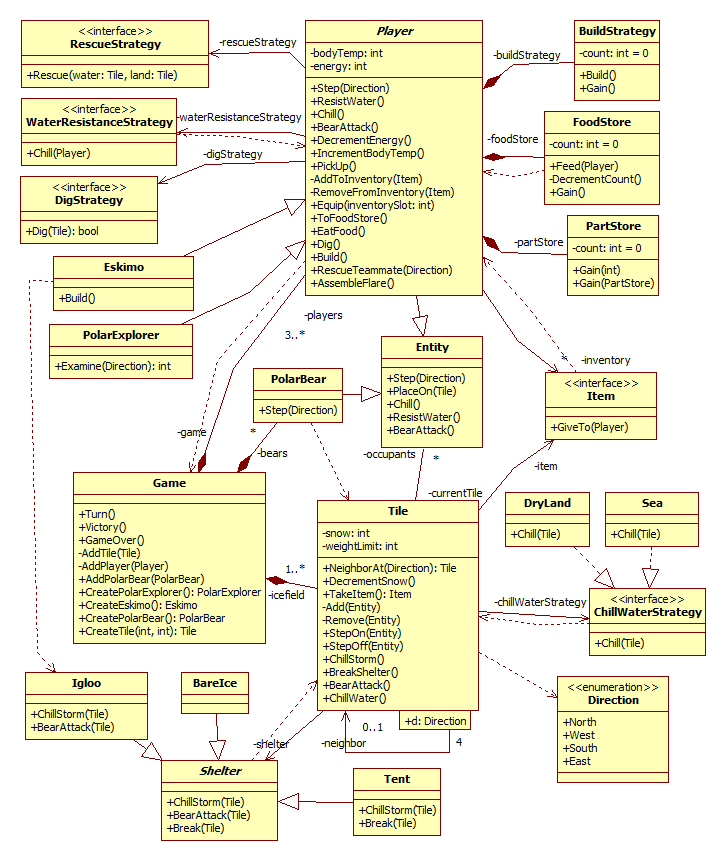
\includegraphics[angle=90, scale=0.76]{chapters/chapter07/ClassDiagramPart1.png}
		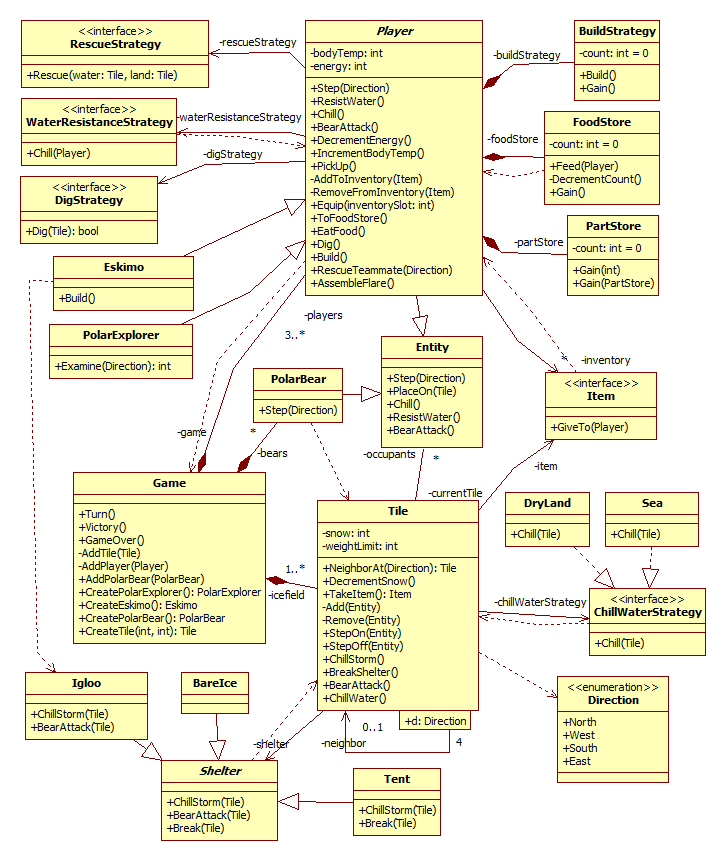
\includegraphics[width=18cm]{chapters/chapter07/ClassDiagramPart1.png}
		\caption{Osztálydiagram 1.}
		\label{fig:OsztalyDiagramPart1}
	\end{center}
\end{figure}
\begin{figure}[H]
	\begin{center}
		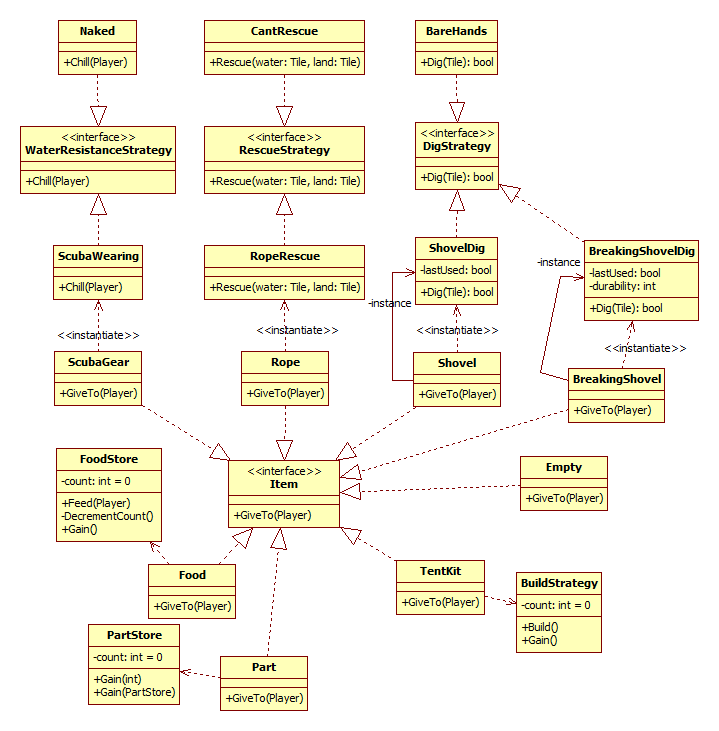
\includegraphics[width=17cm]{chapters/chapter07/ClassDiagramPart2.png}
		\caption{Osztálydiagram 2.}
		\label{fig:OsztalyDiagramPart2}
	\end{center}
\end{figure}

Új osztályok
\begin{itemize}
\item BreakingShovel
	\begin{itemize}
	\item implements Item
	\item Törékeny lapát tárgy.
	\end{itemize}
\item BreakingShovelDig
	\begin{itemize}
	\item implements DigStrategy
	\item Így ásnak a törékeny lapáttal.
	\end{itemize}
\item BuildStrategy
	\begin{itemize}
	\item A játékos így épít sátrat.
	\end{itemize}
\item Direction
	\begin{itemize}
	\item Egy irány a pálya négyzetrácson. Észak, dél, kelet, nyugat.
	\end{itemize}
\item Entity
	\begin{itemize}
	\item Egy dolog ami tud lépkedni a jégtáblákon.
	\item A játékosok és a jegesmedve, Entity-k.
	\end{itemize}
\item PolarBear
	\begin{itemize}
	\item implements Entity
	\item Megtámadja a játékosokat, akikkel találkozik.
	\end{itemize}
\item Shelter
	\begin{itemize}
	\item Egy jégtábla ilyen védelmet nyújt a rajta álló játékosoknak a medve és a vihar elől.
	\end{itemize}
\item Tent
	\begin{itemize}
	\item implements Shelter.
	\item Sátor.
	\end{itemize}
\item TentKit
	\begin{itemize}
	\item implements Item
	\item Ezzel a tárggyal lehet sátrat építeni.
	\end{itemize}
\end{itemize}

\subsection{Új vagy megváltozó metódusok}
%\comment{Az analízis modell osztályleírásaiból azon metódusok újbóli felsorolása leírással együtt, amelyek a változtatás miatt módosultak vagy újonnan be lettek vezetve.}
\begin{itemize}
\item Shelter.ChillStorm(Tile)
\begin{itemize} \item A paraméterként kapott Tilen lévő összes játékos fázik, meghívódik a Chill metódusuk. \end{itemize}

\item Shelter.BearAttack(Tile)
\begin{itemize} \item A paraméterként kapott Tilen lévő összes játékos elszenvedi a medvetámadást, meghívódik a BearAttack metódusuk.  \end{itemize}

\item Shelter.Break(Tile)
\begin{itemize} \item A metódus visszatér, nem csinál semmit, azért van, hogy leszármazottak felüldefiniálják. \end{itemize}

\item Igloo.ChillStorm()
\begin{itemize} \item A metódus visszatér, mert az igluban a játékosok nem fáznak. \end{itemize}

\item Igloo.BearAttack()
\begin{itemize} \item A metódus visszatér, mert az iglu véd a medvétől. \end{itemize}

\item Tile.ChillStorm()
\begin{itemize} \item A rajta lévő Shelter menedék ChillStorm metódusát hívja a hóviharban. \end{itemize}

\item Entity.Chill() 
\begin{itemize} \item A metódus visszatér, nem csinál semmit, azért van, hogy leszármazottak felüldefiniálják. \end{itemize}

\item Entity.ResistWater()
\begin{itemize} \item A metódus visszatér, nem csinál semmit, azért van, hogy leszármazottak felüldefiniálják. \end{itemize}

\item Entity.BearAttack()
\begin{itemize} \item A metódus visszatér, nem csinál semmit, azért van, hogy leszármazottak felüldefiniálják. \end{itemize}

\item Entitiy.Step(direction)
\begin{itemize} \item Az entitás lekéri a jelenlegi mezőjétől a mezőt, ami a paraméterként kapott irányban van, a jelenlegi mezőről lelép, átlép az újra. \end{itemize}

\item Entity.PlaceOn(t: Tile)
\begin{itemize} \item Az entitás a paraméterként kapott Tilere lép, beállítódik currentTile-jének az. \end{itemize}

\item Player.Step(direction)
\begin{itemize} \item A játékos energiája csökken, majd ősosztálya lépés metódusa hívódik, ugyanazt csinálja. \end{itemize}

\item Tile.BreakShelter()
\begin{itemize} \item A kör elején a jégtábla megpróbálja eltörni a rajta lévő menedéket, meghívva annak a Break metódusát. Nem minden menedék törik el, a Break metódus felüldefiniálásától függ ez végül. \end{itemize}

\item Tent.Break(t: Tile)
\begin{itemize} \item A sátor eltörik a kör elején, ezért a sátor halálát úgy jelzi, hogy a paraméterként kapott jégtábla(amin a sátor van) menedékét sima jégre beállítja. \end{itemize}

\item Tent.ChillStorm()
\begin{itemize} \item A metódus visszatér, mert a sátorban nem fázik az ember. \end{itemize}

\item TentKit.GiveTo(p: Player)
\begin{itemize} \item  A paraméterként kapott játékos kap a BuildStrategyjébe egy sátrat. p.BuildStrategy.IncrementCount() és kiveszi magát az inventoryból, mert consumable. \end{itemize}

\item BuildStrategy.Build(t:Tile)
\begin{itemize} \item  Eggyel fogy az építhető sátrak száma, majd a paraméterként kapott Tilere épül egy sátor. \end{itemize}

\item Player.Build()
\begin{itemize} \item A játékos energiája eggyel fogy, majd a megfelelő építési stratégiája függvényében épít a jelenlegi mezőjére. \end{itemize}

\item Eskimo.Build()
\begin{itemize} \item Az eszkimó energiája fogy eggyel, majd épít egy iglut a jelenlegi mezőjére. Nem érdekli őt, hogy van-e nála sátor, az iglu úgyis jobb. \end{itemize}

\item Game.initplayer
\begin{itemize} \item  A Game.CreateEskimo és a Game.CreatePolarExplorer közös részszekvenciája. A playernek ad egy BuildStrategyt, 0-ás számlálóval \end{itemize}

\item Game.Turn()
\begin{itemize} \item  A játékban új kör kezdődik, a játékosok energiája feltölt, ott meghívódik annak a metódusa, a vízben lévő  játékosok fáznak, a jégtáblákon lévő menedékek megpróbálnak eltörni. \end{itemize}

\item BreakingShovel.GiveTo(p: Player)
\begin{itemize} \item A paraméterként kapott Player megfelelő stratégiája helyére bekerül az eltörésre képes lapát, emellett az inventoryjába is. A lapát megjegyzi hány durabilityje van, és csak annyi ásást engedélyez a játékosnak eltörés előtt. \end{itemize}

\item BreakingShovelDig.Dig()
\begin{itemize} \item A lapát durabilityje csökken, minden második ásásra tér vissza igazzal, hogy egy energiával a játékos tudjon kettőt ásni. Ha a lapát eltört, a játékos mindenképp fárad, és nem ás ki havat a jégtábláról, egyébként igen. \end{itemize}

\item Game.CreatePolarBear()
\begin{itemize} \item A játék létrehoz egy jegesmaci objektumot, leteszi egy mezőre, hogy onnantól elinduljon véletlenszerű útján. \end{itemize}

\item PolarBear.Step(direction)
\begin{itemize} \item A paraméterként kapott irányba lép a jegesmaci, az ősosztálya lépéséhez hasonlóan, az ős lépés metódusa hívódik meg. A mezőt, amire rálépett, meg is támadja, hiszen falatozni akar az ízletes játékosok puha húsából. \end{itemize}

\item Player.BearAttack()
\begin{itemize} \item Ha egy játékost megtámadott a medve, nem tud védekezni ellene. Meghal, és a játék véget ér. \end{itemize}

\item Tile.BearAttack()
\begin{itemize} \item Az adott mezőt megtámadta a medve, ezért az szól a rajta lévő menedéknek, hogy megtámadta a medve, tegyen valamit. A menedék attól függően, hogy hogy definiálja felül a BearAttack(Tile) metódusát, védi meg, vagy hagyja meghalni az ott lévő játékosokat. \end{itemize}

\item Game.CreateTile(snow, weightLimit)
\begin{itemize} \item Ez a függvény a játék jégtáblagenerálásáért felel. A paraméterként kapott hó és teherbírásmennyiség függvénéyben generál jégtáblát, majd azt összekapcsolja szomszédaival. Ez a metódus majd a tesztelés során lesz nagyon hasznos. \end{itemize}

\end{itemize}


\subsection{Szekvencia-diagramok}

% TODO: labelezni, captionozni
% TODO: width-et állítani

\begin{figure}[H]
        \begin{center}
                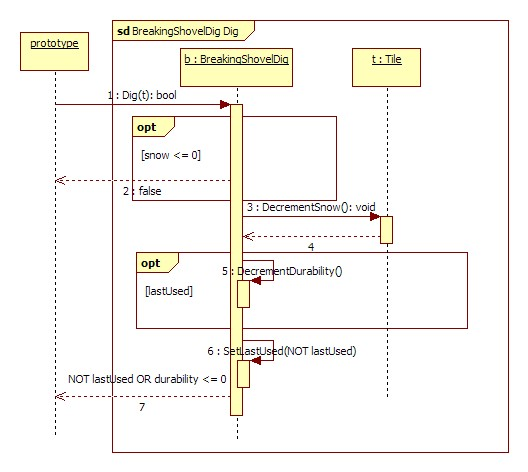
\includegraphics[width=10cm]{chapters/chapter07/seqdiag/BreakingShovelDig_Dig.jpg}
                \caption{BreakingShovelDig Dig}
                \label{BreakingShovelDig Dig}
        \end{center}
\end{figure}
\begin{figure}[H]
        \begin{center}
                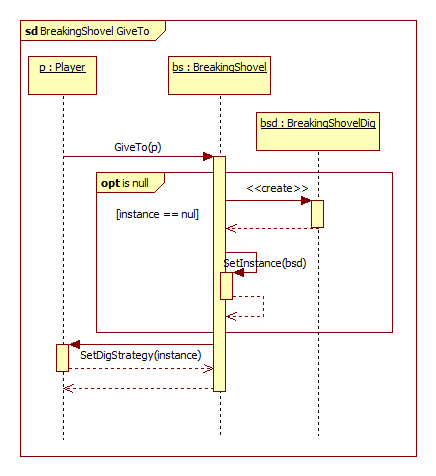
\includegraphics[width=10cm]{chapters/chapter07/seqdiag/BreakingShovel_GiveTo.png}
                \caption{BreakingShovel GiveTo}
                \label{BreakingShovel GiveTo}
        \end{center}
\end{figure}
\begin{figure}[H]
        \begin{center}
                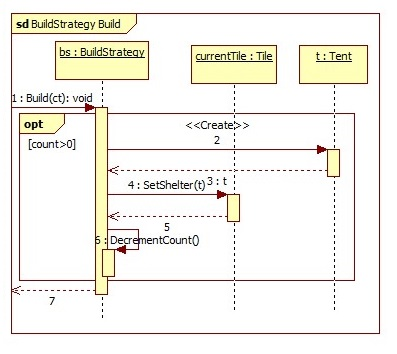
\includegraphics[width=10cm]{chapters/chapter07/seqdiag/BuildStrategy_Build.jpg}
                \caption{BuildStrategy Build}
                \label{BuildStrategy Build}
        \end{center}
\end{figure}
\begin{figure}[H]
        \begin{center}
                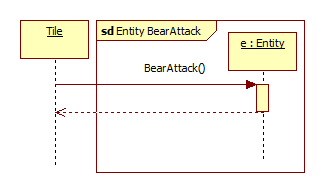
\includegraphics[width=10cm]{chapters/chapter07/seqdiag/Entity_BearAttack.png}
                \caption{Entity BearAttack}
                \label{Entity BearAttack}
        \end{center}
\end{figure}
\begin{figure}[H]
        \begin{center}
                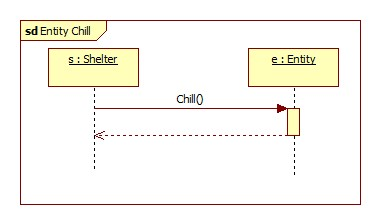
\includegraphics[width=10cm]{chapters/chapter07/seqdiag/Entity_Chill.jpg}
                \caption{Entity Chill}
                \label{Entity Chill}
        \end{center}
\end{figure}
\begin{figure}[H]
        \begin{center}
                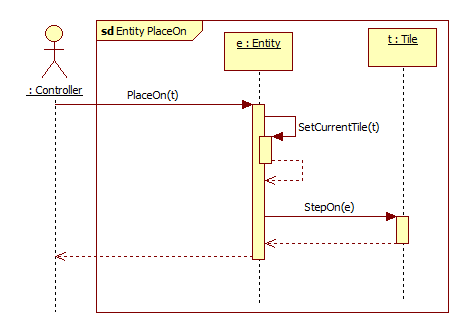
\includegraphics[width=10cm]{chapters/chapter07/seqdiag/Entity_PlaceOn.png}
                \caption{Entity PlaceOn}
                \label{Entity PlaceOn}
        \end{center}
\end{figure}
\begin{figure}[H]
        \begin{center}
                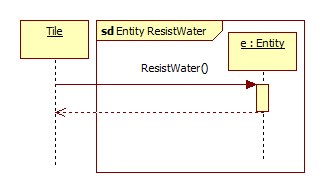
\includegraphics[width=10cm]{chapters/chapter07/seqdiag/Entity_ResistWater.png}
                \caption{Entity ResistWater}
                \label{Entity ResistWater}
        \end{center}
\end{figure}
\begin{figure}[H]
        \begin{center}
                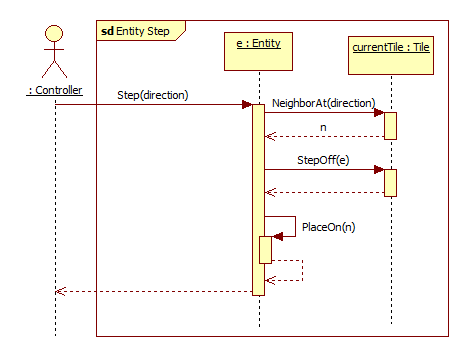
\includegraphics[width=10cm]{chapters/chapter07/seqdiag/Entity_Step.png}
                \caption{Entity Step}
                \label{Entity Step}
        \end{center}
\end{figure}
\begin{figure}[H]
        \begin{center}
                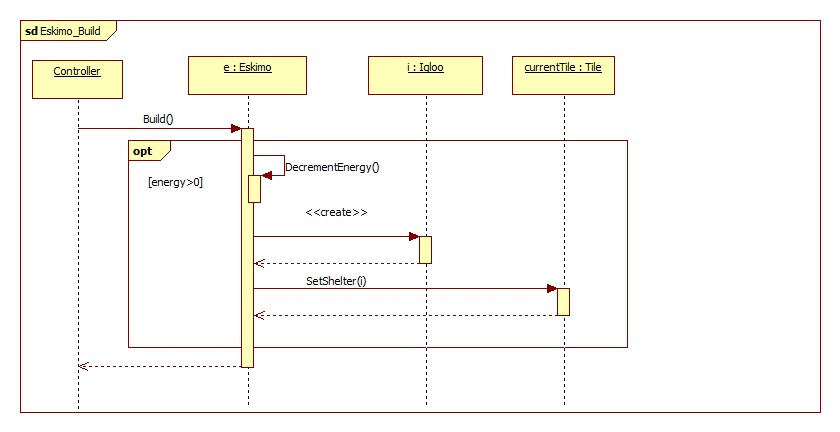
\includegraphics[width=10cm]{chapters/chapter07/seqdiag/Eskimo_Build.jpg}
                \caption{Eskimo Build}
                \label{Eskimo Build}
        \end{center}
\end{figure}
\begin{figure}[H]
        \begin{center}
                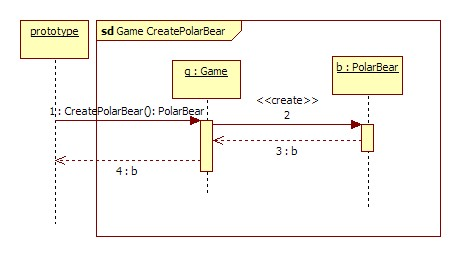
\includegraphics[width=10cm]{chapters/chapter07/seqdiag/Game_CreatePolarBear.jpg}
                \caption{Game CreatePolarBear}
                \label{Game CreatePolarBear}
        \end{center}
\end{figure}
\begin{figure}[H]
        \begin{center}
                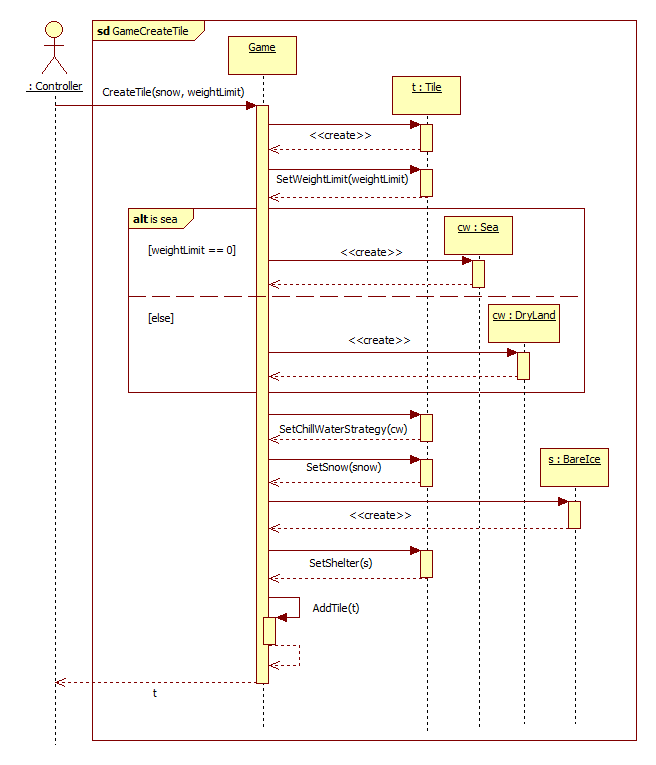
\includegraphics[width=10cm]{chapters/chapter07/seqdiag/Game_CreateTile.png}
                \caption{Game CreateTile}
                \label{Game CreateTile}
        \end{center}
\end{figure}
\begin{figure}[H]
        \begin{center}
                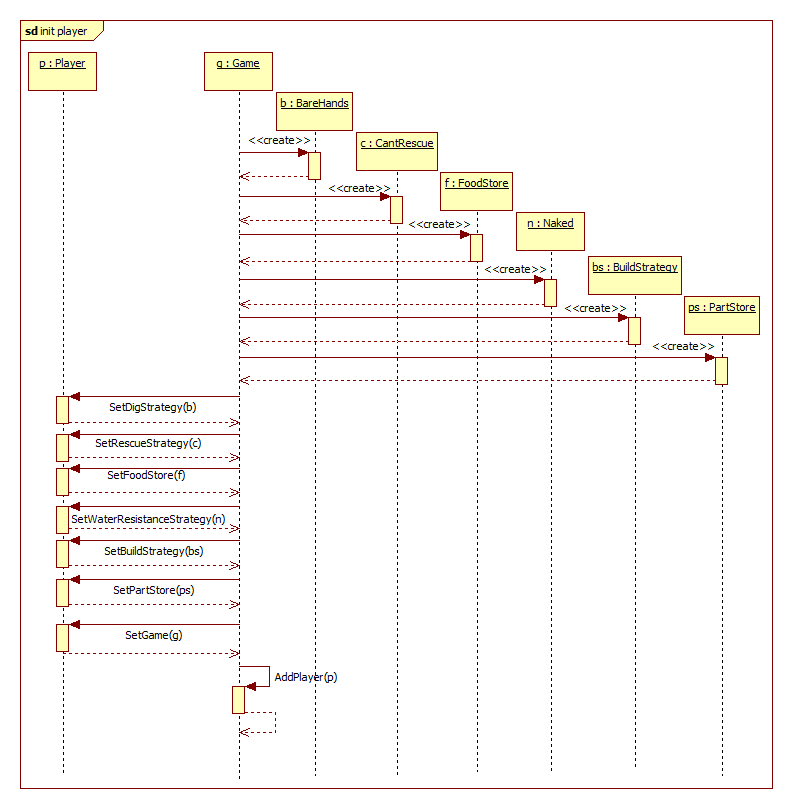
\includegraphics[width=10cm]{chapters/chapter07/seqdiag/Game_init_player.png}
                \caption{Game init player}
                \label{Game init player}
        \end{center}
\end{figure}
\begin{figure}[H]
        \begin{center}
                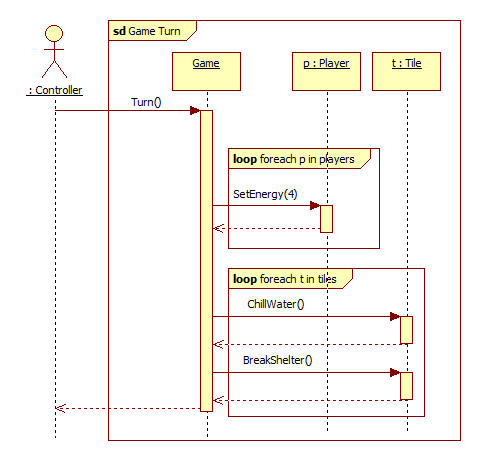
\includegraphics[width=10cm]{chapters/chapter07/seqdiag/Game_Turn.png}
                \caption{Game Turn}
                \label{Game Turn}
        \end{center}
\end{figure}
\begin{figure}[H]
        \begin{center}
                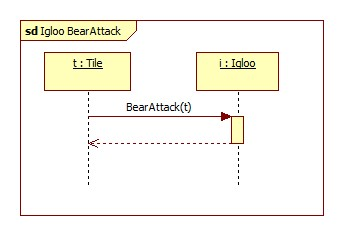
\includegraphics[width=10cm]{chapters/chapter07/seqdiag/Igloo_BearAttack.jpg}
                \caption{Igloo BearAttack}
                \label{Igloo BearAttack}
        \end{center}
\end{figure}
\begin{figure}[H]
        \begin{center}
                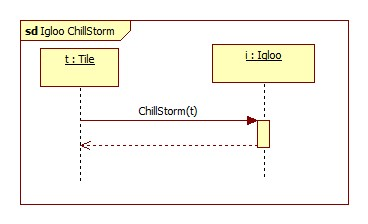
\includegraphics[width=10cm]{chapters/chapter07/seqdiag/Igloo_ChillStorm.jpg}
                \caption{Igloo ChillStorm}
                \label{Igloo ChillStorm}
        \end{center}
\end{figure}
\begin{figure}[H]
        \begin{center}
                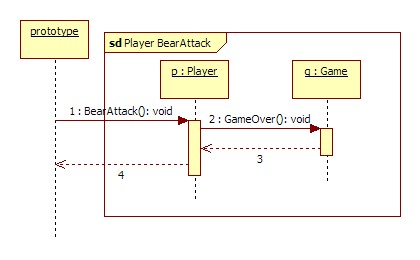
\includegraphics[width=10cm]{chapters/chapter07/seqdiag/Player_BearAttack.jpg}
                \caption{Player BearAttack}
                \label{Player BearAttack}
        \end{center}
\end{figure}
\begin{figure}[H]
        \begin{center}
                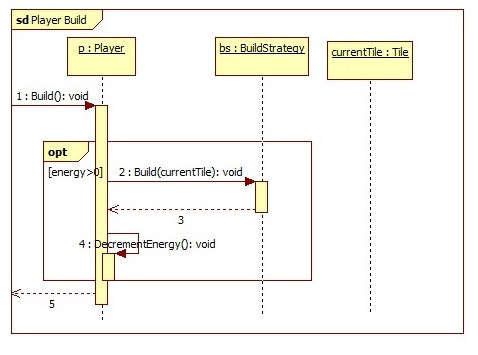
\includegraphics[width=10cm]{chapters/chapter07/seqdiag/Player_Build.jpg}
                \caption{Player Build}
                \label{Player Build}
        \end{center}
\end{figure}
\begin{figure}[H]
        \begin{center}
                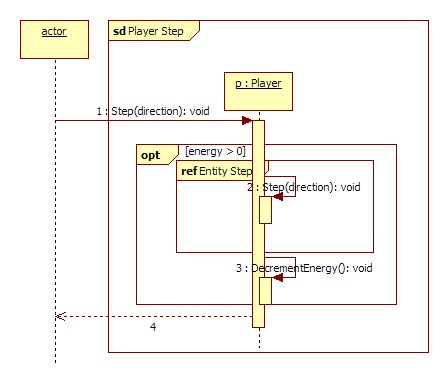
\includegraphics[width=10cm]{chapters/chapter07/seqdiag/Player_Step.jpg}
                \caption{Player Step}
                \label{Player Step}
        \end{center}
\end{figure}
\begin{figure}[H]
        \begin{center}
                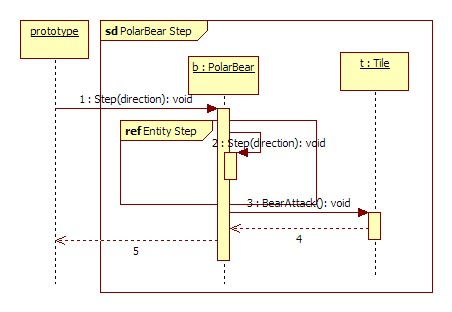
\includegraphics[width=10cm]{chapters/chapter07/seqdiag/PolarBear_Step.jpg}
                \caption{PolarBear Step}
                \label{PolarBear Step}
        \end{center}
\end{figure}
\begin{figure}[H]
        \begin{center}
                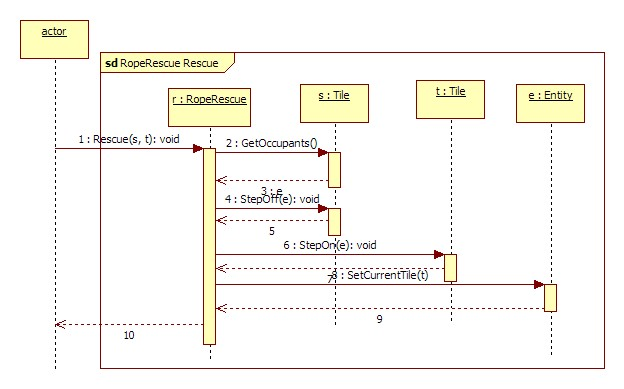
\includegraphics[width=10cm]{chapters/chapter07/seqdiag/RopeRescue_Rescue.jpg}
                \caption{RopeRescue Rescue}
                \label{RopeRescue Rescue}
        \end{center}
\end{figure}
\begin{figure}[H]
        \begin{center}
                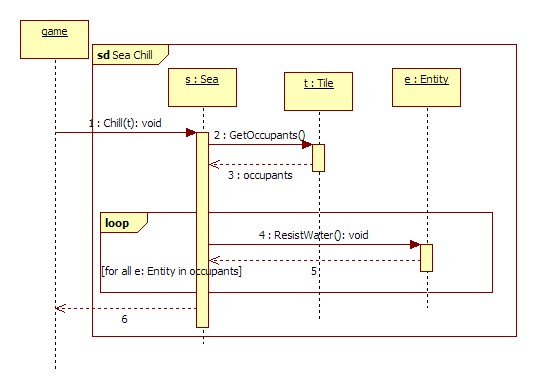
\includegraphics[width=10cm]{chapters/chapter07/seqdiag/Sea_Chill.jpg}
                \caption{Sea Chill}
                \label{SeaChill}
        \end{center}
\end{figure}
\begin{figure}[H]
        \begin{center}
                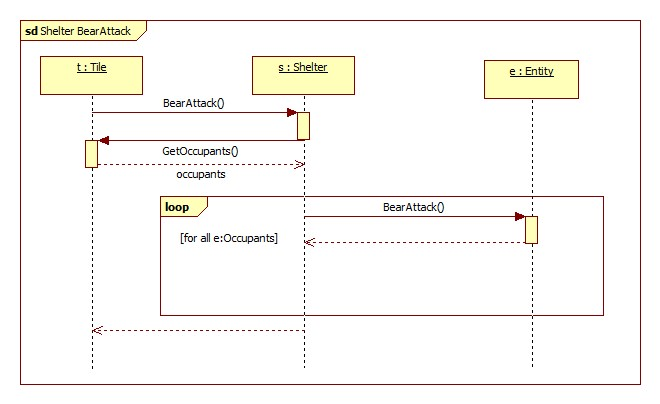
\includegraphics[width=10cm]{chapters/chapter07/seqdiag/Shelter_BearAttack.jpg}
                \caption{Shelter BearAttack}
                \label{Shelter BearAttack}
        \end{center}
\end{figure}
\begin{figure}[H]
        \begin{center}
                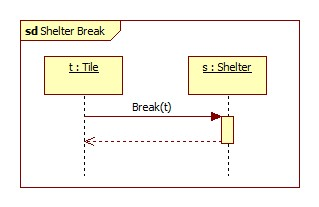
\includegraphics[width=10cm]{chapters/chapter07/seqdiag/Shelter_Break.jpg}
                \caption{Shelter Break}
                \label{Shelter Break}
        \end{center}
\end{figure}
\begin{figure}[H]
        \begin{center}
                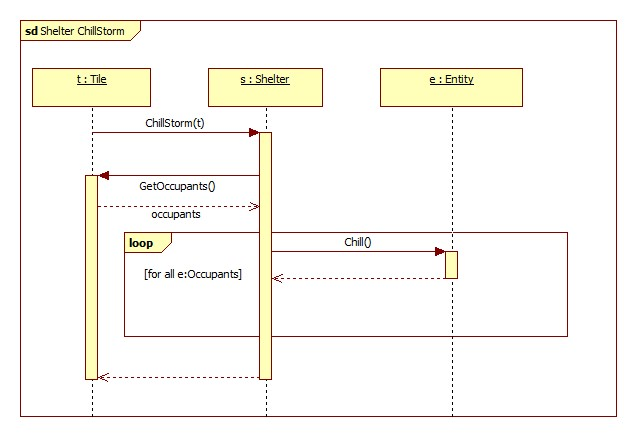
\includegraphics[width=10cm]{chapters/chapter07/seqdiag/Shelter_ChillStorm.jpg}
                \caption{Shelter ChillStorm}
                \label{Shelter ChillStorm}
        \end{center}
\end{figure}
\begin{figure}[H]
        \begin{center}
                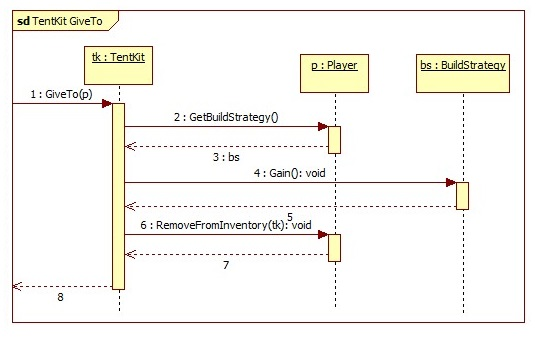
\includegraphics[width=10cm]{chapters/chapter07/seqdiag/TentKit_GiveTo.jpg}
                \caption{TentKit GiveTo}
                \label{TentKit GiveTo}
        \end{center}
\end{figure}
\begin{figure}[H]
        \begin{center}
                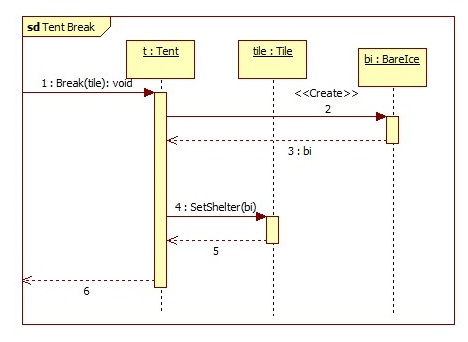
\includegraphics[width=10cm]{chapters/chapter07/seqdiag/Tent_Break.jpg}
                \caption{Tent Break}
                \label{Tent Break}
        \end{center}
\end{figure}
\begin{figure}[H]
        \begin{center}
                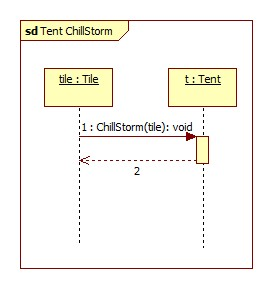
\includegraphics[width=10cm]{chapters/chapter07/seqdiag/Tent_ChillStorm.jpg}
                \caption{Tent ChillStorm}
                \label{Tent ChillStorm}
        \end{center}
\end{figure}
\begin{figure}[H]
        \begin{center}
                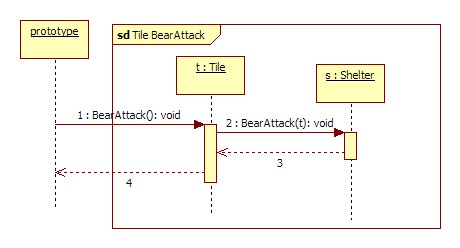
\includegraphics[width=10cm]{chapters/chapter07/seqdiag/Tile_BearAttack.jpg}
                \caption{Tile BearAttack}
                \label{Tile BearAttack}
        \end{center}
\end{figure}
\begin{figure}[H]
        \begin{center}
                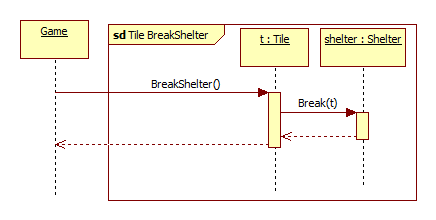
\includegraphics[width=10cm]{chapters/chapter07/seqdiag/Tile_BreakShelter.png}
                \caption{Tile BreakShelter}
                \label{Tile BreakShelter}
        \end{center}
\end{figure}
\begin{figure}[H]
        \begin{center}
                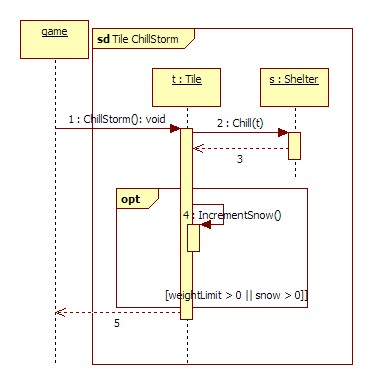
\includegraphics[width=10cm]{chapters/chapter07/seqdiag/Tile_ChillStorm.jpg}
                \caption{Tile ChillStorm}
                \label{Tile ChillStorm}
        \end{center}
\end{figure}
\begin{figure}[H]
        \begin{center}
                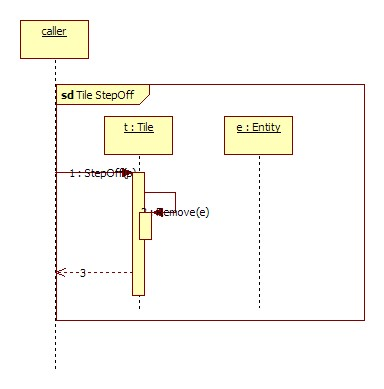
\includegraphics[width=10cm]{chapters/chapter07/seqdiag/Tile_StepOff.jpg}
                \caption{Tile StepOff}
                \label{Tile StepOff}
        \end{center}
\end{figure}
\begin{figure}[H]
        \begin{center}
                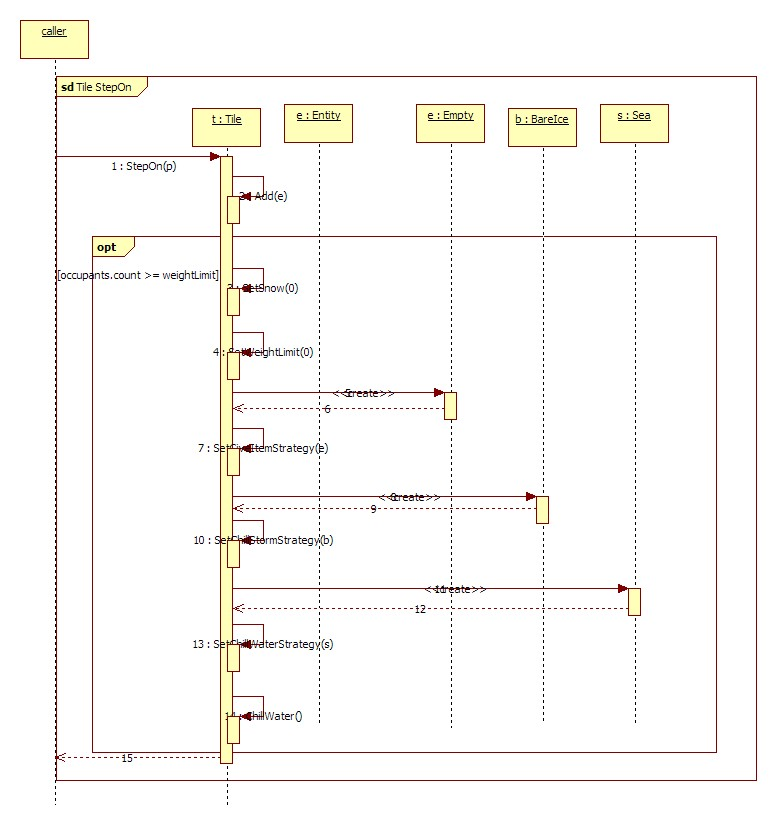
\includegraphics[width=10cm]{chapters/chapter07/seqdiag/Tile_StepOn.jpg}
                \caption{Tile StepOn}
                \label{Tile StepOn}
        \end{center}
\end{figure}

\section{Prototípus interface-definíciója}
%\comment{Definiálni kell a teszteket leíró nyelvet. Külön figyelmet kell fordítani arra, hogy ha a rendszer véletlen elemeket is tartalmaz, akkor a véletlenszerűség ki-bekapcsolható legyen, és a program determinisztikusan is tesztelhető legyen.}

\subsection{Az interfész általános leírása}
%\comment{A protó (karakteres) input és output felületeit úgy kell kialakítani, hogy az input fájlból is vehető legyen illetőleg az output fájlba menthető legyen, vagyis kommunikációra csak a szabványos be- és kimenet használható.}
A program egysoros parancsokat vár a standard bemeneten. A játék kezdőállapotát definíciós parancsokkal kell megadni, majd vezérő parancsokkal lehet játszani. A \texttt{query} speciális parancs hatására, a játék teljes jelenlegi állapota kiíródik a standard kimenetre, definíciós parancsok sorozataként.

\subsection{Bemeneti nyelv}
%\comment{Definiálni kell a teszteket leíró nyelvet. Külön figyelmet kell fordítani arra, hogy ha a rendszer véletlen elemeket is tartalmaz, akkor a véletlenszerűség ki-bekapcsolható legyen, és a program determinisztikusan is futtatható legyen. A szálkezelést is tesztelhető, irányítható módon kell megoldani.}

\definecolor{mymaroon}{rgb}{0.5, 0.07, 0}
\definecolor{myblue}{rgb}{0, 0.02, 0.9}
\lstset{
	breakatwhitespace=false,
	keepspaces=false,
	breaklines=true,
	frame=L,
	numbers=left,
	language=C, %kicsit hasonlít a C-re
	basicstyle=\small\ttfamily,
	identifierstyle=\color{myblue},
	stringstyle=\color{mymaroon},
	caption={A program által elfogadott bemeneti nyelvtan Extended Backus-Naur formában.},
	label=GrammarEBNF
}
\lstinputlisting{chapters/chapter07/grammar.ebnf}

Szótár:

\begin{itemize}
\item \texttt{action\textunderscore{}command}
A jelenleg kiválasztott játékos cselekvése.
\item \texttt{assemble\textunderscore{}command}
A jelenleg kiválasztott játékos összeszereli a rakétát.
\item \texttt{build\textunderscore{}command}
A jelenleg kiválasztott játékos iglut/sátrat épít.
\item \texttt{building\textunderscore{}command}
A jelenleg kiválasztott cellára iglu/sátor épül.
\item \texttt{building\textunderscore{}type}
Iglu vagy sátor.
\item \texttt{command\textunderscore{}end}
Parancsok közti karaktersorozat, amit nem értelmezünk.
\item \texttt{comment}
\# karaktertől a sor végéig lehet komment.
\item \texttt{connect\textunderscore{}command}
A jelenleg kiválasztott cella szomszédaihoz adja az adott cellá(ka)t.
\item \texttt{dig\textunderscore{}command}
A jelenleg kiválasztott játékos havat lapátol.
\item \texttt{entity\textunderscore{}command}
Egy entitás létrehozása.
\item \texttt{entity\textunderscore{}definition}
Egy entitás létrehozása és tulajdonságainak beállítása.
\item \texttt{equip\textunderscore{}all\textunderscore{}command}
A jelenleg kiválasztott játékos felveszi az összes birtokában lévő tárgyat.
\item \texttt{equip\textunderscore{}command}
A jelenleg kiválasztott játékos felvesz birtokában lévő tárgyat.
\item \texttt{equip\textunderscore{}index}
Egy - játékos által birtokolt - tárgy száma.
\item \texttt{equip\textunderscore{}index\textunderscore{}command}
A jelenleg kiválasztott játékos felveszi az adott birtokában lévő tárgyat.
\item \texttt{examine\textunderscore{}command}
A jelenleg kiválasztott sarkkutató játékos felderít egy cellát.
\item \texttt{game}
Parancsok helyes sorozata.
\item \texttt{integer}
Nemnegatív egész szám, tízes számrendszerben.
\item \texttt{item\textunderscore{}command}
Tárgy/Tárgyak létrehozása.
\item \texttt{item\textunderscore{}command\textunderscore{}multiple}
Több tárgy létrehozása.
\item \texttt{item\textunderscore{}command\textunderscore{}single}
Egy tárgy létrehozása.
\item \texttt{item\textunderscore{}count}
Tárgyak számának megadása.
\item \texttt{item\textunderscore{}durability}
A törékeny lapát tárgy hátramaradt használásainak száma.
\item \texttt{item\textunderscore{}type}
Tárgy megadása.
\item \texttt{map\textunderscore{}definition}
A pálya létrehozása.
\item \texttt{pickup\textunderscore{}command}
A jelenleg kiválasztott játékos kiás egy tárgyat a jégből.
\item \texttt{player\textunderscore{}actions}
Egy játékos cselekedetei.
\item \texttt{player\textunderscore{}bodyheat}
Egy játékos testhője.
\item \texttt{player\textunderscore{}class}
Játékos osztály megadása: eszkimó/sarkkutató.
\item \texttt{player\textunderscore{}command}
Egy játékos létrehozása.
\item \texttt{player\textunderscore{}definition}
Egy játékos létrehozása, és birtokolt tárgyainak beállítása.
\item \texttt{player\textunderscore{}energy}
Játékos hátramaradt energiája.
\item \texttt{player\textunderscore{}equipped\textunderscore{}items}
Ezeket a tárgyakat a játékos felveszi.
\item \texttt{player\textunderscore{}index}
Játékos száma.
\item \texttt{player\textunderscore{}inventory\textunderscore{}items}
Ezek a tárgyak a játékos birtokába kerülnek.
\item \texttt{polarbear\textunderscore{}actions}
A jelenleg kiválasztott jegesmedve cselekedetei.
\item \texttt{polarbear\textunderscore{}command}
A jelenleg kiválasztott jegesmedve létrehozása.
\item \texttt{polarbear\textunderscore{}index}
Jegesmedve száma.
\item \texttt{query\textunderscore{}command}
A parancs hatására \texttt{map\textunderscore{}definition} íródik ki az stdout-ra, ami reprezentálja a játék jelenlegi állapotát.
\item \texttt{rescue\textunderscore{}command}
A jelenleg kiválasztott játékos kíhúzza csapattársát a vízből.
\item \texttt{select\textunderscore{}tile\textunderscore{}command}
Kiválaszt egy cellát.
\item \texttt{select\textunderscore{}player\textunderscore{}command}
Kiválaszt egy játékost.
\item \texttt{select\textunderscore{}polarbear\textunderscore{}command}
Kiválaszt egy jegesmedvét.
\item \texttt{step\textunderscore{}command}
A jelenleg kiválasztott játékos lép.
\item \texttt{storm\textunderscore{}command}
Hóvihar kezdődik.
\item \texttt{tile\textunderscore{}command}
Egy cella létrehozása.
\item \texttt{tile\textunderscore{}definition}
Egy cella létrehozása, és a rajta lévő dolgok létrehozása.
\item \texttt{tile\textunderscore{}snow}
A cella hószintjének definiálása.
\item \texttt{tile\textunderscore{}topology}
A cella szomszédainak beállítása.
\item \texttt{tile\textunderscore{}weight\textunderscore{}limit}
A cella teherbírásának definiálása: hány entitás állhat rajta. \newline A * karakter végtelen teherbírást jelöl. A 0 teherbírású cella tenger.
\item \texttt{turn\textunderscore{}command}
A parancs hatására új kör kezdődik a játékban.
\item \texttt{turn\textunderscore{}definition}
Egy kör során végrehajtott parancsok sorozata.
\end{itemize}

%\comment{Ha szükséges, meg kell adni a konfigurációs (pl. pályaképet megadó) fájlok nyelvtanát is.}

\subsection{Kimeneti nyelv}
%\comment{Egyértelműen definiálni kell, hogy az egyes bemeneti parancsok végrehajtása után előálló állapot milyen formában jelenik meg a szabványos kimeneten.}
A kimeneti nyelv a bemeneti nyelv részhalmaza. Pontosabban, egy  \texttt{map\textunderscore{}definition} nyelvi elem. Kivételes esetek a következők:
\begin{itemize}
\item Sarkkutató felderít egy cellát.
	\begin{itemize}
	\item Az \texttt{examine\textunderscore{}command} lefutását követően üzenet jelenik meg a standard kimeneten: \newline \texttt{"Tile weight limit: N\textbackslash{}n"}, ahol N a cella teherbírása.
	\end{itemize}
\item Egy játékos meghal.
	\begin{itemize}
	\item Üzenet jelenik meg: \texttt{"Game over.\textbackslash{}n"}, és a program megáll.
	\end{itemize}
\item A játékosok összeszerelik a rakétát.
	\begin{itemize}
	\item Üzenet jelenik meg: \texttt{"Victory.\textbackslash{}n"}, és a program megáll.
	\end{itemize}
\end{itemize}

\section{Összes részletes use-case}
%\comment{A use-case-eknek a részletezettsége feleljen meg a kezelői felületnek, azaz a felület elemeire kell hivatkozniuk. Alábbi táblázat minden use-case-hez külön-külön.}

\begin{figure}[h]
\begin{center}
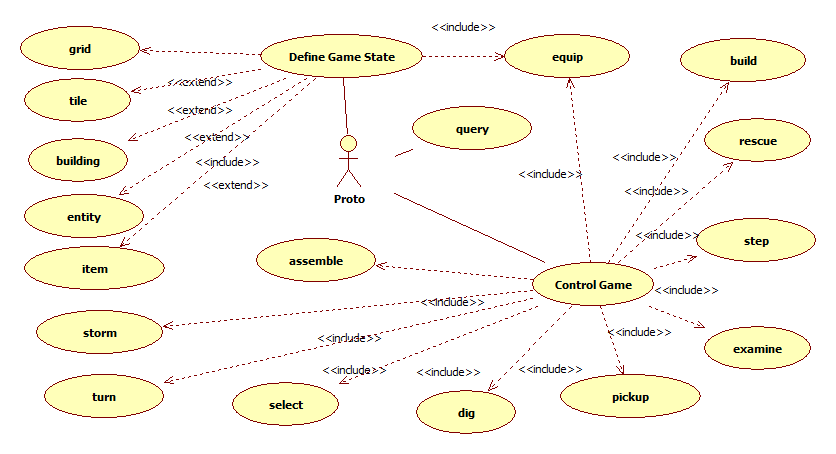
\includegraphics[width=17cm]{chapters/chapter07/ProtoUseCases.png}
\caption{Use-case diagram}
\label{fig:ProtoUseCases}
\end{center}
\end{figure}

% TODO
\newpage % ha ez nincs, akkor a diagram beketül a táblázatok közé
% de így is bugos, mert egy-két táblázat lecsúszik a lapról

%\usecase{grid}{Pályaméret beállítása.}{Proto}{
%	1. Jön egy \texttt{grid\textunderscore{}command}.\newline
%	2. A pályaméret beállítódik.
%}
\usecase{tile}{Cella létrehozása.}{Proto}{
	1. Jön egy \texttt{tile\textunderscore{}command}.\newline
	2. Létrejön az adott cella.
}
\usecase{building}{Épület létrehozása.}{Proto}{
	1. Jön egy \texttt{building\textunderscore{}command}.\newline
	2. Létrejön az adott épület.
}
\usecase{item}{Tárgy létrehozása.}{Proto}{
	1. Jön egy \texttt{item\textunderscore{}command}.\newline
	2. Létrejön az adott tárgy, vagy tárgyak.
}
\usecase{equip}{Tárgy felvétele.}{Proto}{
	1. Jön egy \texttt{equip\textunderscore{}command}.\newline
	2. A jelenleg kiválasztott játékos felvesz egy tárgyat.
}
\usecase{entity}{Entitás létrehozása.}{Proto}{
	1. Jön egy \texttt{entity\textunderscore{}command}.\newline
	2. Létrejön az adott entitás.
}
\usecase{select}{Entitás kiválasztása.}{Proto}{
	1. Jön egy \texttt{select\textunderscore{}command}.\newline
	2. Kiválasztódik az adott entitás
}
\usecase{turn}{Új kör kezdése.}{Proto}{
	1. Jön egy \texttt{turn\textunderscore{}command}.\newline
	2. Új kör kezdődik.
}
\usecase{storm}{Vihar kezdése.}{Proto}{
	1. Jön egy \texttt{storm\textunderscore{}command}.\newline
	2. Vihar kezdődik.
}
\usecase{step}{Entitás lép.}{Proto}{
	1. Jön egy \texttt{step\textunderscore{}command}.\newline
	2. A jelenleg kiválasztott entitás lép.
}
\usecase{rescue}{Játékos megment.}{Proto}{
	1. Jön egy \texttt{rescue\textunderscore{}command}.\newline
	2. A jelenleg kiválasztott játékos kíhúzza csapattársát a vízből.
}
\usecase{dig}{Játékos lapátol.}{Proto}{
	1. Jön egy \texttt{dig\textunderscore{}command}.\newline
	2. A jelenleg kiválasztott játékos lapátol.
}
\usecase{pickup}{Játékos felvesz.}{Proto}{
	1. Jön egy \texttt{pickup\textunderscore{}command}.\newline
	2. A jelenleg kiválasztott játékos kiás egy tárgyat.
}
\usecase{build}{Játékos épít.}{Proto}{
	1. Jön egy \texttt{build\textunderscore{}command}.\newline
	2. A jelenleg kiválasztott játékos épít.
}
\usecase{assemble}{Játékos összeszerel}{Proto}{
	1. Jön egy \texttt{assemble\textunderscore{}command}.\newline
	2. A jelenleg kiválasztott játékos összeszereli a rakétát.
}
\usecase{examine}{Jégtábla felderítése}{Proto}{
	1. Jön egy \texttt{examine\textunderscore{}command}.\newline
	2. A jelenleg kiválasztott sarkkutató játékos felderít egy mezőt.
}
\usecase{query}{A játékállapot lekérdezése.}{Proto}{
	1. Jön egy \texttt{query\textunderscore{}command}.\newline
	2. A játék állapota kiíródik a standard kimenetre.
}

\section{Tesztelési terv}
%\comment{A tesztelési tervben definiálni kell, hogy a be- és kimeneti fájlok egybevetésével miként végezhető el a program tesztelése. Meg kell adni teszt forgatókönyveket. Az egyes teszteket elég informálisan, szabad szövegként leírni. Teszt-esetenként egy-öt mondatban. Minden teszthez meg kell adni, hogy mi a célja, a proto mely funkcionalitását, osztályait stb. teszteli. Az alábbi táblázat minden teszt-esethez külön-külön elkészítendő.}

\teszteset{PickUpFood}{A játékos az adott mezőre lép. A mezőn élelem található. A játékos felveszi és a saját zsebébe rakja az ételt.}{Item felvétel teszt.}
\teszteset{PickUpPart}{A játékos adott mezőre lép. A mezőn rakéta pisztoly darab található. A játékos felveszi és a megfelelő zsebébe rakja.}{Item felvétel teszt.}
\teszteset{PickUpShovel}{A játékos adott mezőre lép. A mezőn ásó található. A játékos felvesz és a zsebébe rakja. A játékos ez utána már tud ásni később.}{Item felvétel teszt.}
\teszteset{PickUpBreakableShovel}{A játékos adott mezőre lép. A mezőn törékeny ásó található. A játékos felvesz és a zsebébe rakja. A játékos ez utána már tud ásni később.}{Item felvétel teszt.}
\teszteset{PickUpRope}{A játékos adott mezőre lép. A mezőn kötél található. A játékos felvesz és a zsebébe rakja. A játékos ez utána már ki tudja menteni a csapattársait.}{Item felvétel teszt.}
\teszteset{PickUpScubaGear}{A játékos adott mezőre lép. A mezőn búvárruha található. A játékos felvesz és a zsebébe rakja. A játékos ez utána már képes túlélni a vízben.}{Item felvétel teszt.}
\teszteset{PickUpTent}{A játékos adott mezőre lép. A mezőn sátor található. A játékos felvesz és a zsebébe rakja. A játékos ez utána már képes sátrat építeni egy mezőre.}{Item felvétel teszt.}
\teszteset{BareHandsDig}{A játékos azon a mezőn ahol éppen áll havat lapátol. A hómennyiség az adott mezőn csökken}{Hó lapátolás.}
\teszteset{ShovelDig}{A játékos azon a mezőn ahol éppen áll havat lapátol, van nála lapát. A hómennyiség az adott mezőn csökken}{Hó lapátolás.}
\teszteset{BreakingShovelDig}{A játékos azon a mezőn ahol éppen áll havat lapátol, van nála törékeny lapát. A hómennyiség az adott mezőn csökken. A lapát még nem törik el.}{Hó lapátolás.}
\teszteset{BreakingShovelDig}{A játékos azon a mezőn ahol éppen áll havat lapátol, van nála törékeny lapát. A hómennyiség az adott mezőn csökken. A lapát eltörik}{Hó lapátolás.}
\teszteset{StepOnStableIce}{A játékos stabil jégre lép.}{Játékos mezőre lép.}
\teszteset{StepOnUnstableIceWithScubaGearBreaking}{A játékos instabil jégre lép. A játékoson van búvárruha. A jég eltörik, mert nem bírja el. Minden játékos vízbe esik aki ott volt.}{Játékos mezőre lép.}
\teszteset{StepOnUnstableIceWithScubaGearCanHold}{A játékos instabil jégre lép. A játékoson van búvárruha. A jég nem törik el.}{Játékos mezőre lép.}
\teszteset{StepOnUnstableIceNakedBreaking}{A játékos instabil jégre lép. A játékoson nincs búvárruha. A jég eltörik, mert nem bírja el. Minden játékos vízbe esik aki ott volt.}{Játékos mezőre lép.}
\teszteset{StepOnUnstableIceNakedCanHold}{A játékos instabil jégre lép. A játékoson nincs búvárruha. A jég nem törik el.}{Játékos mezőre lép.}
\teszteset{StepInWaterWithScubaGear}{A játékos víz mezőre lép. A játékoson van búvárruha. A játékos kibírja a vízbe esést.}{Játékos mezőre lép.}
\teszteset{StepInWaterNaked}{A játékos víz mezőre lép. A játékoson nincs búvárruha.A játékos meg fog fagyni, ha nem mentik ki később.}{Játékos mezőre lép.}
\teszteset{RopeRescue}{A játékosnak van kötele. Egy játékos kiment egy másik játékost a vízből és a saját táblájára húzza.}{Játékos cselekszik}
\teszteset{EatFood}{A játékosnak van élelme. A játékos elfogyaszt 1 élelmet a zsebéből és nő a testhője.}{Játékos cselekszik.}
\teszteset{AssembleFlare}{A játékosnál van az összes rakéta darab. A játékos összeszereli azt.}{Játékos cselekszik.}
\teszteset{AssembleFlareFail}{A játékosnál nincs meg az összes rakéta darab és megpróbálja összeszerelni a pisztolyt.}{Játékos cselekszik.}
\teszteset{BuildIgloo}{Az eszkimó felvesz egy TentKit-et. Az eszkimó a táblára iglut épít, nem pedig sátrat.}{Tábla esemény teszt.}
\teszteset{BuildTent}{A sarkkutató felvesz egy TentKit-et. A sarkkutató a táblára sátrat épít.}{Tábla esemény teszt.}
\teszteset{ExamineTile}{A sarkkutató a táblát vizsgálja.}{Tábla esemény teszt.}
\teszteset{TurnOnStableIce}{Egy játék kör eltelik úgy, hogy a játékos a stabil jégen áll.}{Játék esemény teszt.}
\teszteset{TurnInWaterNaked}{Egy játék kör eltelik úgy, hogy a játékos vízben áll. A játékoson van búvárruha.}{Játék esemény teszt.}
\teszteset{TurnInWaterWithScubaGear}{Egy játék kör eltelik úgy, hogy a játékos vízben áll. A játékoson nincs búvárruha.}{Játék esemény teszt.}
\teszteset{ChillStormIgloo}{Egy játék kör eltelik, úgy, hogy a játékost hóvihar éri. A játékos igluban van.}{Játék esemény teszt.}
\teszteset{ChillStormTent}{Egy játék kör eltelik, úgy, hogy a játékost hóvihar éri. A játékos sátorban van.}{Játék esemény teszt.}
\teszteset{ChillStormBareIce}{Egy játék kör eltelik, úgy, hogy a játékost hóvihar éri. A játékos szabad ég alatt van.}{Játék esemény teszt.}
\teszteset{TentBreaking}{A táblán a sátor eltörik a kör után.}{Játék esemény teszt.}
\teszteset{PolarBearMoving}{A medve véletlen irányba lép. Üres mezőre lép.}{Játék esemény teszt.}
\teszteset{PolarBearAttack}{A medve véletlen irányba lép. A mezőn van valaki.}{Játék esemény teszt.}
\teszteset{PolarBearAttackTent}{A medve véletlen irányba lép. A mezőn sátorban van valaki.}{Játék esemény teszt.}
\teszteset{PolarBearAttackIgloo}{A medve véletlen irányba lép. A mezőn igluban van valaki.}{Játék esemény teszt.}

\section{Tesztelést támogató segéd- és fordítóprogramok specifikálása}
%\comment{Specifikálni kell a tesztelést támogató segédprogramokat.}
Nincs.

